\documentclass[a4paper,10pt]{article}
\usepackage[utf8]{inputenc}
\usepackage{natbib}

\usepackage[pdftex]{graphicx}
\usepackage{caption}
\usepackage{subcaption}

\graphicspath{{./images/}}
\DeclareGraphicsExtensions{.pdf,.jpeg,.png,.jpg}
\hyphenation{op-tical net-works semi-conduc-tor}

%\addtolength{\textheight}{2cm}
\addtolength{\textwidth}{2cm}
\addtolength{\hoffset}{-1cm}
%opening
\title{P2P Security - State of the Art\\
Forschungsmethoden WS2012\\
Gruppe 7}
\author{0502196 - Andreas Rohner\\
%0828266 - Murat Dogan\\
%1029102 - Christian Marbach\\
0626885 - Andreas Egger
}

\begin{document}

\maketitle

\begin{abstract}
A P2P approach seems to be the next logical step for many services that have to
scale massivly like VoIP. But a P2P service implies new security challenges
since clients have to rely on untrusted peers. It is difficult to identify
malicious peers without central control. This paper describes a selection of
possible security threats in this
environment, and then discusses some approaches, presented in the scientific
literature, to ameliorate them. Since the list of possible threats is extensive,
this paper focuses on threats that require some kind of user interaction.
\end{abstract}

\section{Introduction}

P2P applications face a number of security threats, because it has
to rely on untrusted and possibly malicious peers to provide the service.

Furthermore private data such as offline messages and voice mails have to be
stored in the overlay network and therefore on untrusted peers, who can
deny access to it or return fake content. Contact information, such as the
current ip address of the node, and other metadata is typically stored in the
overlay network as well.

In the case of a P2P VoIP application, a malicious peer who is
responsible for storing that kind of information could log all incoming calls or
prevent the user from getting any calls at all
\cite{touceda}.

% In section \ref{relatedwork} related work is discussed and
% section \ref{p2p} gives an overview of P2P VoIP in general and of a selection
% of possible attacks. \textsc{Touceda et al.} \cite{touceda} provide a recent
% complete survey of this
% topic. There are numerous possible attacks of the P2P overlay and the impact
% of most attacks can be mitigated by a carefully designed system, but for the
% purpose of this paper especially those attacks,
% that require some kind of user interaction, were chosen. In section
% \ref{usablesecurity} a new approach to mobile security proposed by
% \textsc{Toninelli et al.} \cite{toninelli} is discussed
%  and the findings of \textsc{Koskela et al.} \cite{koskela} are summarized in
% reference to the attacks presented in section \ref{p2p}. Section
% \ref{conclusion} tries to draw some conclusions.

\section{Related Work}
\label{relatedwork}

\textsc{Lua et al.} \cite{lua} provide a good survey and comparison of available
P2P overlay networks and \textsc{Wallach} \cite{wallach} gives an overview of
security threats
and attacks of P2P systems.

\section{Security Threats for P2P VoIP}
\label{p2p}
In an P2P VoIP network the clients have to rely on untrusted peers to provide
the service. This makes it difficult to identify malicious peers, which can
manipulate
the network or provide false information. This section describes a selection of
security threats, that usually require the users attention.

\subsection{P2P architecture}
\begin{figure}[t]
  %\centering

  \begin{minipage}{.5\textwidth}
    \centering
    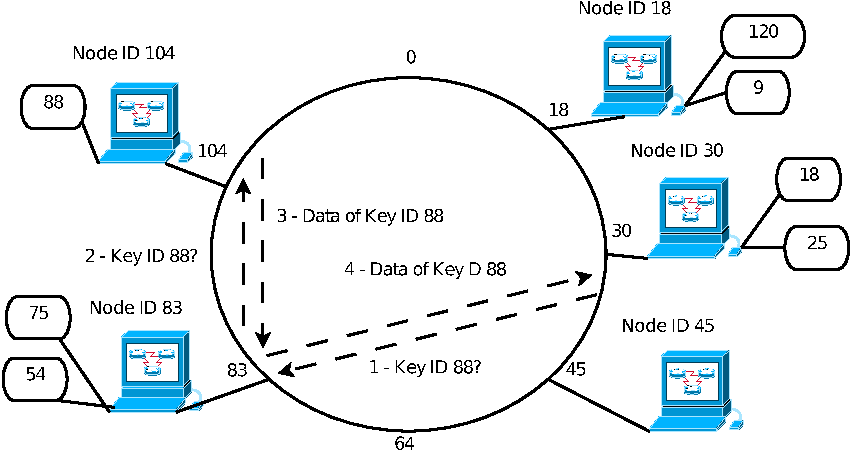
\includegraphics[width=\textwidth]{p2p}
    \caption{P2P overlay network \cite{touceda}}
    \label{fig:p2p}
  \end{minipage}
\hfill
  \begin{minipage}{.5\textwidth}
    \centering
    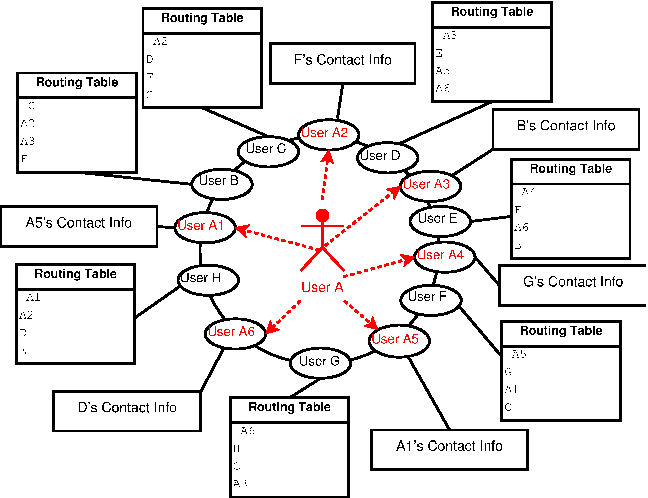
\includegraphics[width=\textwidth]{sybil}
    \caption{Sybil attack where user A controls the network with multiple
    identities \cite{touceda}}
    \label{fig:sybil}
  \end{minipage}

\end{figure}

P2P networks can be classified as either structured or unstructured, whereby the
latter tend to be relatively simple with inefficient searching and the former
use
a distributed hash table (DHT) \cite{chopra}. For the purposes of VoIP a
structured approach seems to be more appropriate because an
efficient lookup is needed. So the attacks described in this section assume a
structured overlay network.


Usually a hash function is used to hash keys into the key space, which is formed
by all possible results of the hash function. Every participant of the overlay
network has a unique random id, which determines the part of the key space it is
responsible for. The ids are of the same size
as the output of the hash function. If a peer wants to store a key value pair in
the DHT it sends the value to the peer, whose id is nearest to the hashed key.
To lookup a key in the DHT it sends a message to the
node in its routing table, whose id is nearest to the hashed key, which in turn
routes the message to the nearest node in its routing table.
Since every node knows its immediate neighborhood, the node responsible for the
key can be found very quickly.

In figure \ref{fig:p2p} node 30 does a lookup of key 88. It queries the nearest
node in its routing table, which happens to be node 83. Node 83 routes the
request to node 104, which is responsible for key 88 and returns the data for
it.

In a simple design malicious nodes can easily disrupt the routing process or
manipulate the values and therefore most implementations use a
public key infrastructure to encrypt and sign the messages. \textsc{Touceda et
al.} \cite{touceda} provide a very good overview of all possible attacks on P2P
VoIP systems.

\subsection{ID Mapping Attack}
\label{idmap}
Usually a node stores its resources in the overlay network, using the hash of
its username as a key. In a P2P VoIP network mostly the nodes contact
information, but
 also voice mails and offline messages are stored. If a node A wants to contact
another node B it hashes its username and does a lookup to retrieve the
contact information, which is stored at a third possibly malicious node C, whose
id is nearest to the hashed username.

So admission control is the first line of defense and very important for the
whole security of the network \cite{touceda, chopra}.
Because if a node can choose its id freely, it can position itself at an
arbitrary spot in the overlay network and make itself responsible for the
resources of a legitimate node. That way it can easily monitor incoming calls,
deny access to it or return fake information \cite{touceda}. Multiple attackers
could also position themselves in such a way, that they appear in the routing
table of the target node. Thereby they could completely manipulate the target
nodes view
of the network.

A simple solution would be to use the hash of the ip address as node id, but,
apart from being incompatible with NATs, where multiple nodes share a single
public ip,
it would still be possible for an attacker, who has access to a large range of
ips, to find a hash near the target key space. Since the key space
is much larger than the number of nodes it suffices to get an id that is near to
the targets hashed username \cite{touceda}.
Another solution would be to use a central certificate authority, which assigns
the node ids at random and signs them with its private key.


\subsection{Sybil Attack}
\label{sybil}

Even if a user is not allowed to choose his node id freely, if there is no limit
on the number of ids he can obtain, a sybil attack is possible.
In that case one attacker could present itself to the system with an unlimited
number of ids and thereby take over a huge part of the overlay network, by
appearing in the routing tables of legitimate users or controlling their contact
information.
It can be shown, that if there is no central control a sybil attack is always
possible \cite{douceur, touceda}.

In figure \ref{fig:sybil} user A presents himself to the network with multiple
node ids and thereby gets control over all contact information and appears in
the routing tables of all other users multiple times.

To prevent this attack the node id could depend on the ip address, which limits
the number of fake nodes to the number of ip addresses available to the
attacker. But
as stated in section \ref{idmap} this approach comes with its own problems. On
the other hand a central certificate authority could link the
node ids with some personal identification such as passport number or social
security number. But it would prove difficult to explain to the end users
why they are required to identify themselves to the certificate authority.

\subsection{Communications Log Attack}
\label{comlog}
\begin{figure}
\centering
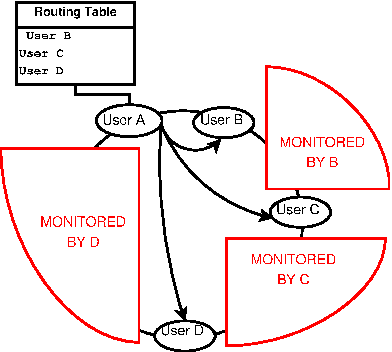
\includegraphics[width=0.5\textwidth]{log}

\caption{Key space which can be monitored by the users in A's routing table
\cite{touceda}}
\label{fig:log}
\end{figure}
Since a node accesses the network through the members of its routing table,
these nodes can monitor all communications. Figure \ref{fig:log} shows a node A
with
nodes B, C and D in its routing table. So
B, C and D can monitor all lookups of A in the key space between them, because A
uses them to route the requests into their respective key spaces. All
nodes on the path from A to the target can also log the message or tamper with
it if it is not encrypted and signed.

As was also noted in section \ref{idmap} an attacker who is responsible for
storing the contact information of a legitimate user can monitor all
incoming calls or deny access to the data, preventing anyone to call the node.

One way to make this attack harder is to use slightly randomized routing
mechanisms, so that not always the same path is chosen. This of course
reduces the efficiency of the routing process. Another way is to obfuscate the
message headers so that they don't reveal anything about the route of
the message \cite{touceda}.
Additionally to prevent an attacker from surrounding a node, id mapping and
sybil attacks described in sections \ref{idmap} and \ref{sybil} respectively
have
to be prevented \cite{touceda}.

Even if all these nodes were trustworthy the contact information of a node is
publicly available and can trivially be accessed through a lookup
\cite{koskelaold}.
So every node in the network can inquire the status of a user and his ip.
Because a P2P network relies on the close cooperation of its participants
it is difficult to provide privacy for the users \cite{koskelaold}.

\subsection{Spam}
\label{spam}
To avoid the same situation as with email, P2P VoIP systems have to be designed
to cope with spam or unsolicited messages and calls. The first step to this end
would be a good admission control as stated in section \ref{idmap} to limit the
number of identities a spam bot can control \cite{touceda}, because, as we see
with email,
if it is easy to obtain or fake new identities, it is hard to prevent spam.
There are three different kinds of spam. Spam over instant messages or SPIM,
spam over
presence protocol or SPPP and spam over ip telephony or SPIT \cite{touceda}.
Whereby SPIT is a much greater disturbance than email spam, because emails can
be filtered based on content on the server before they reach the user, but
unsolicited calls require the immediate attention of the user and cannot be
filtered
based on content until they are answered \cite{heikkilae}. The list below
summarizes some of the more interesting defenses against spam taken from
\cite{touceda}.

\subsubsection{Grey Lists}
If a node contacts another node for the first time it is put on the grey list
and the call is refused with the remark to try again later.
A normal node would try again after a few seconds and the user might not even
notice a difference to a normal call, but a spam bot cannot afford to lose those
seconds per call.
This approach is already known to work well with emails.

\subsubsection{Turing Tests}
To ensure that a human being is behind every call turing tests or CAPTCHAs can
be used. These tests challenge the caller to do something
humans can do, but computers currently cannot. In the case of VoIP, voice based
CAPTCHAs would be used, but any kind
of CAPTCHA would do, such as the distorted images we know from websites.

\subsubsection{Computational Puzzles}
If user A contacts user B, B responds with a computational puzzle and wont
process user A's request until it receives a correct answer \cite{touceda}. Such
puzzles
are difficult to compute, but easy to check, making it computationally expensive
for an attacker to call a large number of addresses in a short time.
But since many different devices with different resources participate in the
network the complexity of these puzzles have to be rather low, which
reduces the effectiveness of this defense.

\subsubsection{Payments at Risk}
If user A calls user B, A transfers a small amount of money to B. If it is a
legitimate call B returns the money, but if it is SPIT B keeps it. Although
the amounts would be very small the accumulated cost of calling thousands of
people would make SPIT very expensive. It is not clear how this money transfer
can reliably work without contacting a central server and thereby losing the
advantages of a decentralized system.

\section{Conclusion}
\label{conclusion}
In this paper a brief introduction into P2P overlay networks, in reference to
P2P VoIP, was given and a summary of some of the attacks, that could exploit
this
architecture followed. Then the usability implications of the defenses and
recent developments in the field of usable security were discussed. It seems,
that
the advantages of a P2P architecture, like scalability and fault tolerance, come
at a price, because the dependence on untrusted peers leaves the user
vulnerable to attacks. Securing P2P networks is a difficult task and an active
field of research. Most of the scientific literature agrees, that at least
some form of central certificate authority, that performs admission control, is
necessary to prevent an attacker from choosing its id freely or get an unlimited
number of fake ids. This measure mitigates many attacks and strengthens the
effectiveness of reputation and social link systems.

\bibliographystyle{plain}
\bibliography{references}

\end{document}
